% \begingroup
% \definecolor{stepfill}{HTML}{F8FAFC}
% \definecolor{stepborder}{HTML}{475569}
% \definecolor{arrowcol}{HTML}{64748B}
% \definecolor{steptext}{HTML}{1E293B}

% \begin{tikzpicture}[
%     >=stealth,
%     execbox/.style={
%         draw=stepborder,
%         fill=stepfill,
%         text=steptext,
%         rounded corners=2pt,
%         line width=0.6pt,
%         text width=6.2cm,
%         minimum height=1.6cm,
%         inner xsep=8pt,
%         inner ysep=6pt,
%         align=center,
%         font=\sffamily\linespread{1}\fontsize{10}{12}\selectfont,
%         execute at begin node={
%             \hyphenpenalty=10000
%             \exhyphenpenalty=10000
%         }
%     },
%     execarrow/.style={
%         ->,
%         draw=arrowcol,
%         line width=0.75pt,
%         shorten <=2pt,
%         shorten >=2pt
%     },
%     execfailure/.style={
%         draw=arrowcol,
%         line width=0.6pt,
%         dashed
%     }
% ]

% \node[execbox] (request) at (0,0)
%     {\textbf{Receive execution request}\\
%      Verification identifier\\
%      Wallet address};

% \node[execbox] (claim) at (0,-2.15)
%     {\textbf{Claim stored approval}\\
%      Check existence, expiry, and reuse\\
%      Retrieve approved operation};

% \node[execbox] (authority) at (0,-4.30)
%     {\textbf{Recheck graph authority}\\
%      Query using saved intent\\
%      Compare approval and current authority};

% \node[execbox] (prepare) at (0,-6.45)
%     {\textbf{Prepare protocol calls}\\
%      Validate parameters and local policy\\
%      Quotes, balances, and allowances};

% \node[execbox] (submit) at (0,-8.60)
%     {\textbf{Submit call batch}\\
%      Kernel smart account\\
%      ZeroDev bundler and paymaster};

% \node[execbox] (result) at (0,-10.75)
%     {\textbf{Return \texttt{EXECUTED}}\\
%      Transaction hash\\
%      Execution summary};

% \node[execbox, text width=2.8cm]
%     (failed) at (7.2,-4.30)
%     {\textbf{Return \texttt{FAILED}}\\
%      Failed check or\\
%      submission error};

% % Main processing path
% \draw[execarrow] (request.south) -- (claim.north);
% \draw[execarrow] (claim.south) -- (authority.north);
% \draw[execarrow] (authority.south) -- (prepare.north);
% \draw[execarrow] (prepare.south) -- (submit.north);
% \draw[execarrow] (submit.south) -- (result.north);

% % Shared failure path
% \draw[execfailure] (4.6,0) -- (4.6,-8.60);

% \draw[execfailure] (request.east) -- (4.6,0);
% \draw[execfailure] (claim.east) -- (4.6,-2.15);
% \draw[execfailure] (authority.east) -- (4.6,-4.30);
% \draw[execfailure] (prepare.east) -- (4.6,-6.45);
% \draw[execfailure] (submit.east) -- (4.6,-8.60);

% \draw[execarrow, dashed]
%     (4.6,-4.30) -- (failed.west);

% \end{tikzpicture}
% \endgroup

\begingroup
\definecolor{stepfill}{HTML}{F8FAFC}
\definecolor{stepborder}{HTML}{475569}
\definecolor{arrowcol}{HTML}{64748B}
\definecolor{steptext}{HTML}{1E293B}

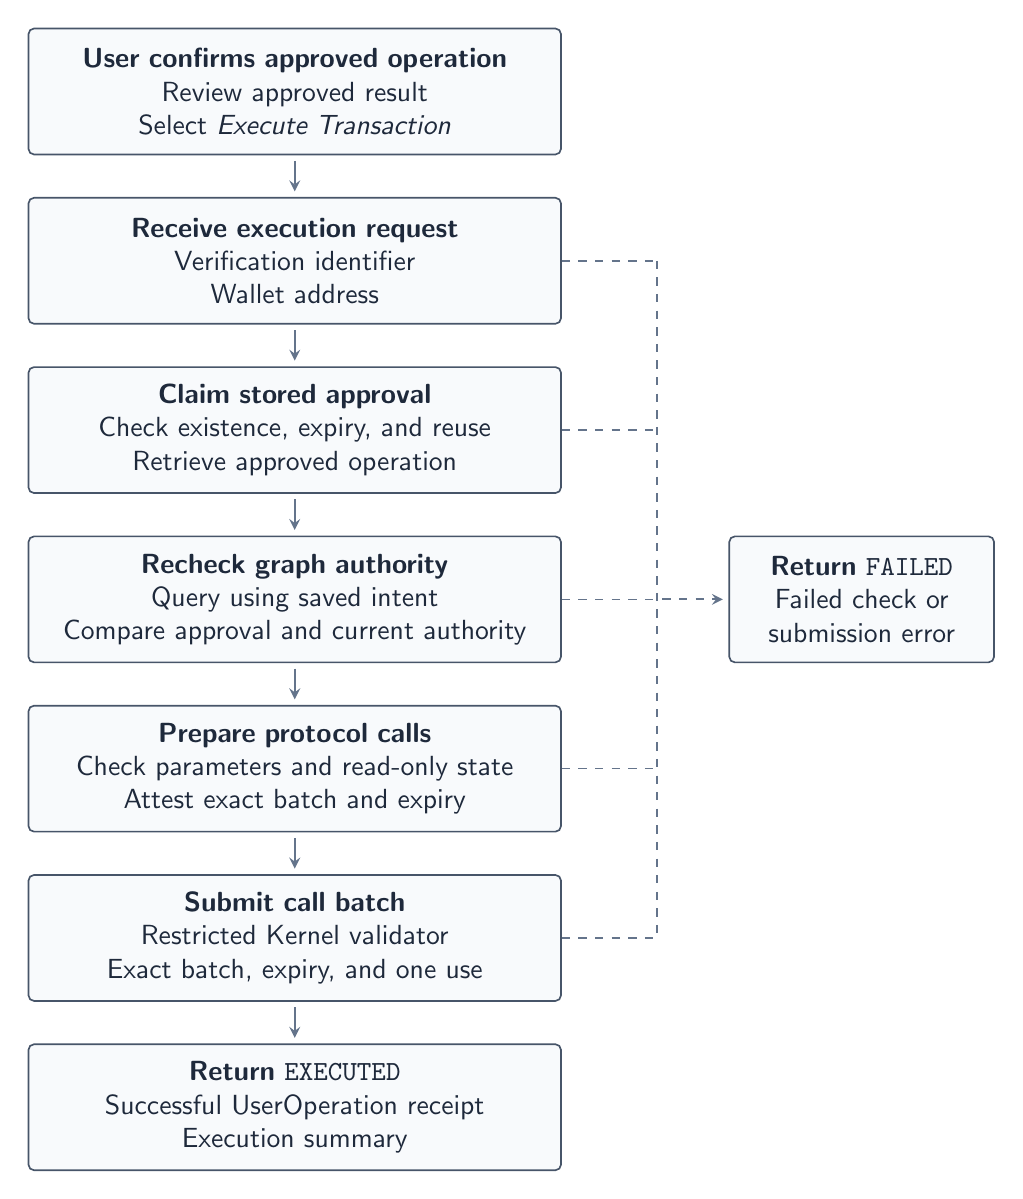
\begin{tikzpicture}[
    >=stealth,
    execbox/.style={
        draw=stepborder,
        fill=stepfill,
        text=steptext,
        rounded corners=2pt,
        line width=0.6pt,
        text width=6.2cm,
        minimum height=1.6cm,
        inner xsep=8pt,
        inner ysep=6pt,
        align=center,
        font=\sffamily\linespread{1}\fontsize{10}{12}\selectfont,
        execute at begin node={
            \hyphenpenalty=10000
            \exhyphenpenalty=10000
        }
    },
    execarrow/.style={
        ->,
        draw=arrowcol,
        line width=0.75pt,
        shorten <=2pt,
        shorten >=2pt
    },
    execfailure/.style={
        draw=arrowcol,
        line width=0.6pt,
        dashed
    }
]

\node[execbox] (approve) at (0,0)
    {\textbf{User confirms approved operation}\\
     Review approved result\\
     Select \textit{Execute Transaction}};

\node[execbox] (request) at (0,-2.15)
    {\textbf{Receive execution request}\\
     Verification identifier\\
     Wallet address};

\node[execbox] (claim) at (0,-4.30)
    {\textbf{Claim stored approval}\\
     Check existence, expiry, and reuse\\
     Retrieve approved operation};

\node[execbox] (authority) at (0,-6.45)
    {\textbf{Recheck graph authority}\\
     Query using saved intent\\
     Compare approval and current authority};

\node[execbox] (prepare) at (0,-8.60)
    {\textbf{Prepare protocol calls}\\
     Check parameters and read-only state\\
     Attest exact batch and expiry};

\node[execbox] (submit) at (0,-10.75)
    {\textbf{Submit call batch}\\
     Restricted Kernel validator\\
     Exact batch, expiry, and one use};

\node[execbox] (result) at (0,-12.90)
    {\textbf{Return \texttt{EXECUTED}}\\
     Successful UserOperation receipt\\
     Execution summary};

\node[execbox, text width=2.8cm]
    (failed) at (7.2,-6.45)
    {\textbf{Return \texttt{FAILED}}\\
     Failed check or\\
     submission error};

% Main processing path
\draw[execarrow] (approve.south) -- (request.north);
\draw[execarrow] (request.south) -- (claim.north);
\draw[execarrow] (claim.south) -- (authority.north);
\draw[execarrow] (authority.south) -- (prepare.north);
\draw[execarrow] (prepare.south) -- (submit.north);
\draw[execarrow] (submit.south) -- (result.north);

% Shared failure path
\draw[execfailure] (4.6,-2.15) -- (4.6,-10.75);

\draw[execfailure] (request.east) -- (4.6,-2.15);
\draw[execfailure] (claim.east) -- (4.6,-4.30);
\draw[execfailure] (authority.east) -- (4.6,-6.45);
\draw[execfailure] (prepare.east) -- (4.6,-8.60);
\draw[execfailure] (submit.east) -- (4.6,-10.75);

\draw[execarrow, dashed]
    (4.6,-6.45) -- (failed.west);

\end{tikzpicture}
\endgroup